%\vspace{-25pt}
\subsubsection{Community Detection}
A community can be defined as a set of nodes that are more densely connected to each other than to the rest of the network. The importance of this approach lies in the fact that nodes that are contained within the same community are expected to share attributes, common characteristics or functional relationships ~\cite{ma2014exploring}.
This work takes advantage of the previously described SQL algorithm in which nodes and relationships are divided to be later visualized by the \texttt{Vis.JS} tool.
In this sense, our approach is based on the search for possible people who participate in criminal gangs. From the data origin it appears that for each node all its relationships can be known, so that we can assign to each of those referring nodes a group or cluster identifier.
It is then possible to verify for each pair of nodes, if they belong to a particular group (one of them will be "referring" and we will be able to identify it), and in this way assign a certain group to each relationship as well. With both tables (nodes and relations) updated, it is possible from the visualization tool to assign colors to each cluster, and thus generate an even more practical graph to view.

Although the JavaScript language is used for visualization by the previously mentioned library \texttt{Vis.JS}, and the datasets are obtained from the System Database \texttt{Coirón} through SQL queries, the software study that takes the data from the dataset and processes it to later call the visualization library, it is developed in the C Sharp language of the .Net Framework.
Below is shown in Figure \ref{fig:graph-10-complete-WithColor} the same visualization that has been presented previously in Figure \ref{fig:graphTop10}, but now with the detection of groups by color. It can be seen that each group or cluster of nodes shares the same color for internal links.
%Una comunidad puede ser definida como un conjunto de nodos que están más densamente conectados entre ellos que con el resto de la red. La importancia de este planteamiento radica en que se espera que los nodos que están contenidos dentro de una misma comunidad compartan atributos, características comunes o relaciones funcionales  ~\cite{ma2014exploring}.
%En este trabajo se aprovecha el algoritmo SQL descrito con anterioridad en el cual se dividen nodos y relaciones para ser luego visualizadas por la herramienta \texttt{Vis.JS}.
%En este sentido, nuestro enfoque se basa en la búsqueda de posibles personas que participen en bandas delictivas. Del origen de datos surge que para cada nodo pueden conocerse todas sus relaciones, de modo que podemos asignar a cada uno de esos nodos referentes un identificador de grupo ó cluster. 
%Es posible entonces verificar para cada par de nodos, si pertenecen a un grupo en particular (uno de ellos será "referente" y podremos identificarlo), y de esta manera asignar a cada relación también un grupo determinado. Con ambas tablas (nodos y relaciones) actualizadas, es posible desde la herramienta de visualización, asignar colores a cada cluster, y así generar un grafo aún más práctico a la vista.

%Si bien para la visualización se utiliza lenguaje JavaScript de la mano de la librería anteriormente mencionada \texttt{Vis.JS}, y los dataset se obtienen desde la Base de Datos del Sistema \texttt{Coirón} a través de consultas SQL, el software de estudio que toma los datos del dataset y los procesa para luego llamar a la librería de visualización, se encuentra desarrollado en lenguaje C Sharp de .Net Framework. 
%A continuación se exhibe en la Figura \ref{fig:grafo-10-completo-ConColor} la misma visualización que se ha presentado con anterioridad en la Figura \ref{fig:grafoTop10}, pero ahora con la detección de grupos por color. Se puede observar que cada grupo o cluster de nodos comparte el mismo color para los enlaces internos. 


%\vspace{-10pt}
\begin{figure}
	\centering
	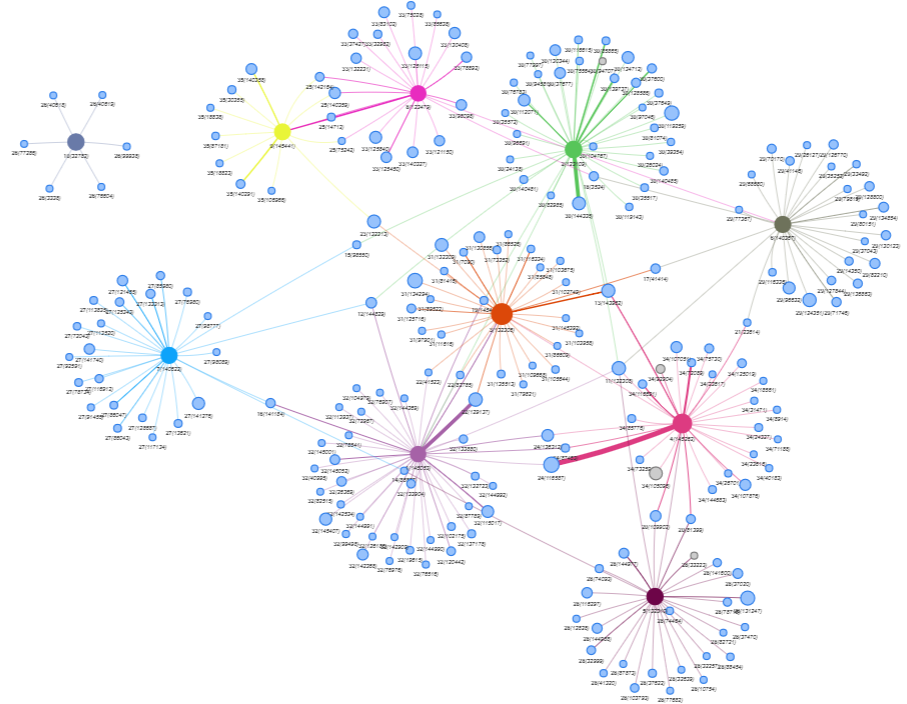
\includegraphics[width=0.5\linewidth]{grafo-10-completo-ConColor.png}
	\caption{10 people with more cases in Coirón, with their relationships. Community detection by color is added.} 
	\label{fig:grafo-10-completo-ConColor}
\end{figure}
%\vspace{-30pt}